\section{Overview}
In this section, we will explain the overall structure of {\germinate} along with an overview of the various data types that {\germinate} supports.

\subsection{Authentication}
{\germinate} can be used with or without user authentication. If the administrator of {\germinate} decided to enable authentication, you will be asked to log in using a username and password. Figure \ref{fig:overview:login} shows the login page of {\germinate}. If you already have a user account, simply enter the username and password into the provided text boxes.

If you do not have a user account, click on the link below the login button to create an account. You may get asked to agree to a license agreement before being able to create an account.

To modify your user account, you can log in to {\gatekeeper}, which is {\germinate}'s user authentication portal. It can be accessed from the help popup on the login page.

\begin{figure}
	\centering
	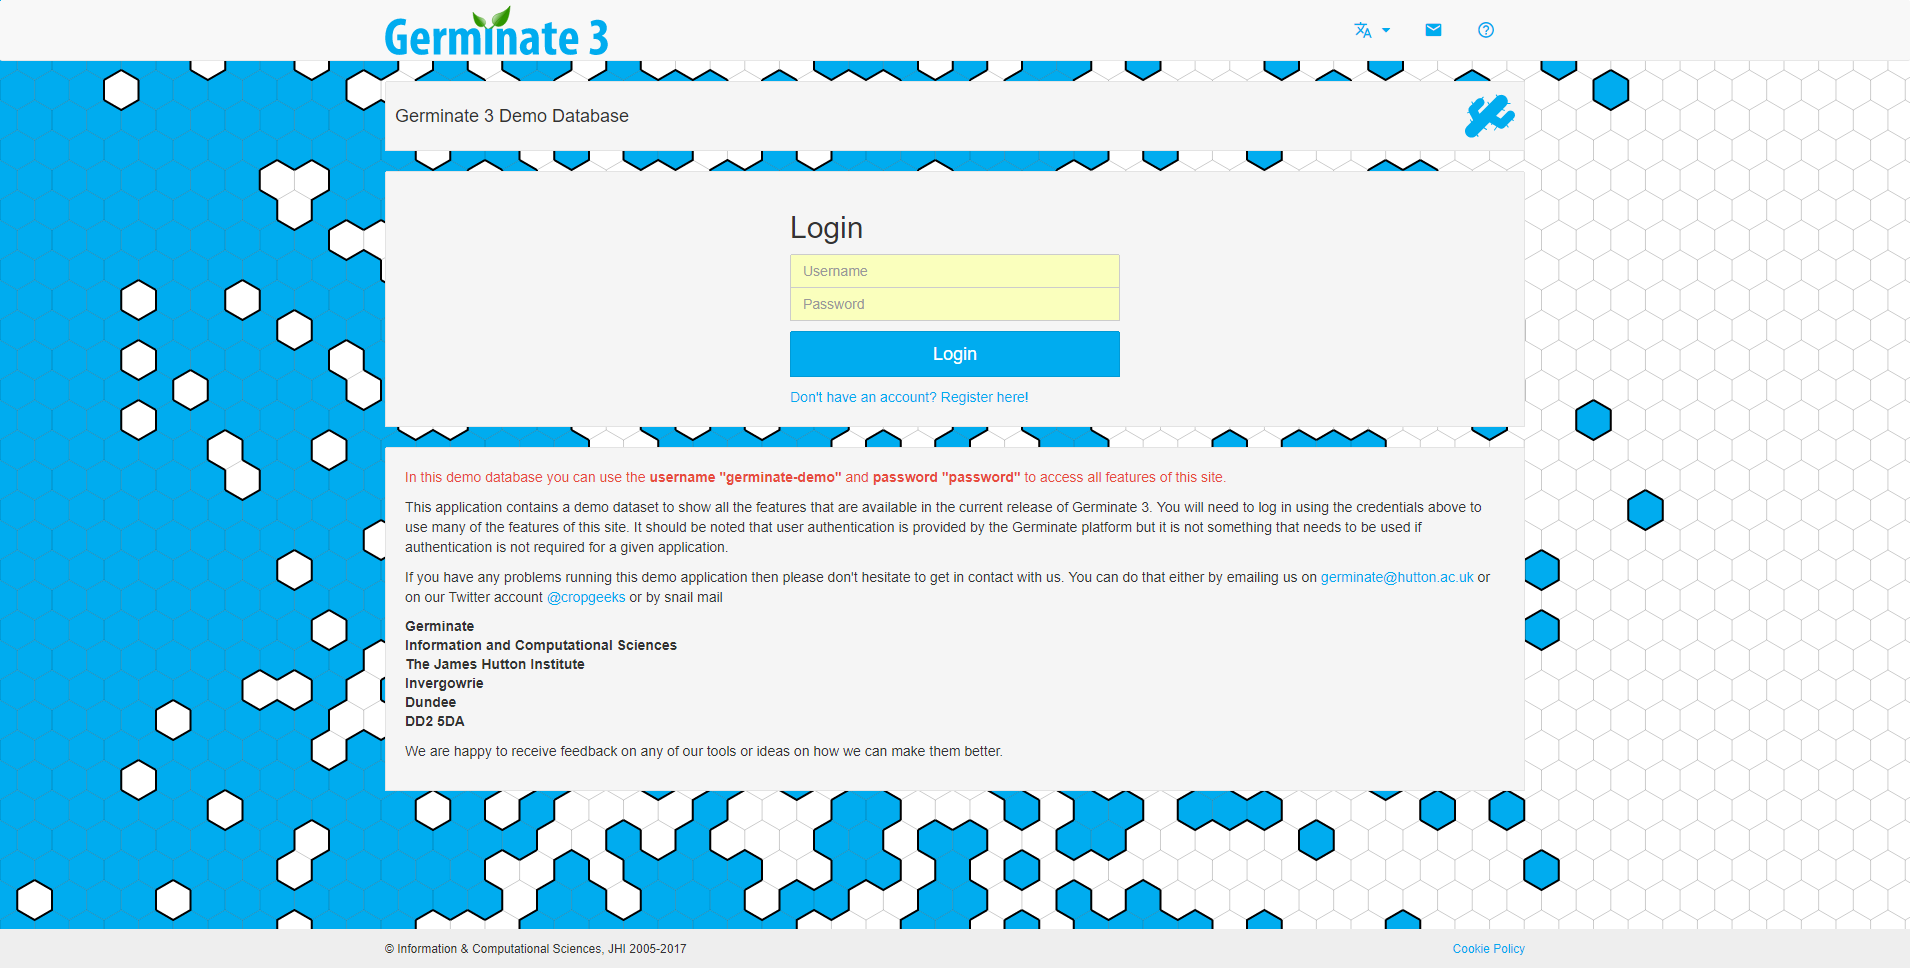
\includegraphics[width=0.85\linewidth]{img/overview/login.png}
	\caption{Depending on the configuration of {\germinate}, you may be asked to log in.}
	\label{fig:overview:login}
\end{figure}

\subsection{Page layout}
Figure \ref{fig:overview:home} shows the main layout of the {\germinate} web interface. The main menu of {\germinate} is positioned to the left (Figure \ref{fig:overview:home}A). It is used to navigate between pages. Submenus can be expanded by simply clicking on the items showing the caret symbol. The menu is explained in more detail in Section \ref{sec:features:menu}. The overall search feature, shown in Figure \ref{fig:overview:home}B, allows you to run a full-text search across the whole database. The results will be grouped into topical categories. See Section \ref{sec:features:search} for more details. The interface has a banner along the top containing the {\germinate} logo and a few dropdown menu items in the top right corner (\cf Figure \ref{fig:overview:home}C). These items include the language selector which will be covered in Section \ref{sec:features:language-selector}, social media buttons, the marked item lists covered in Section \ref{sec:features:marked-items}, a user menu with specific functions based on your type of account, a "contact us" button and, finally, a help button that can be clicked to get more information about the current page (\cf Section \ref{sec:features:help}). An overview of the number of database items for certain types is shown in Figure \ref{fig:overview:home}D. Recent news about both the {\germinate} interface and the contained data are available in the news section shown in Figure \ref{fig:overview:home}E. Finally, a section about other projects that are related to the project you are currently looking at are available in Figure \ref{fig:overview:home}F.

\begin{figure}
	\centering
	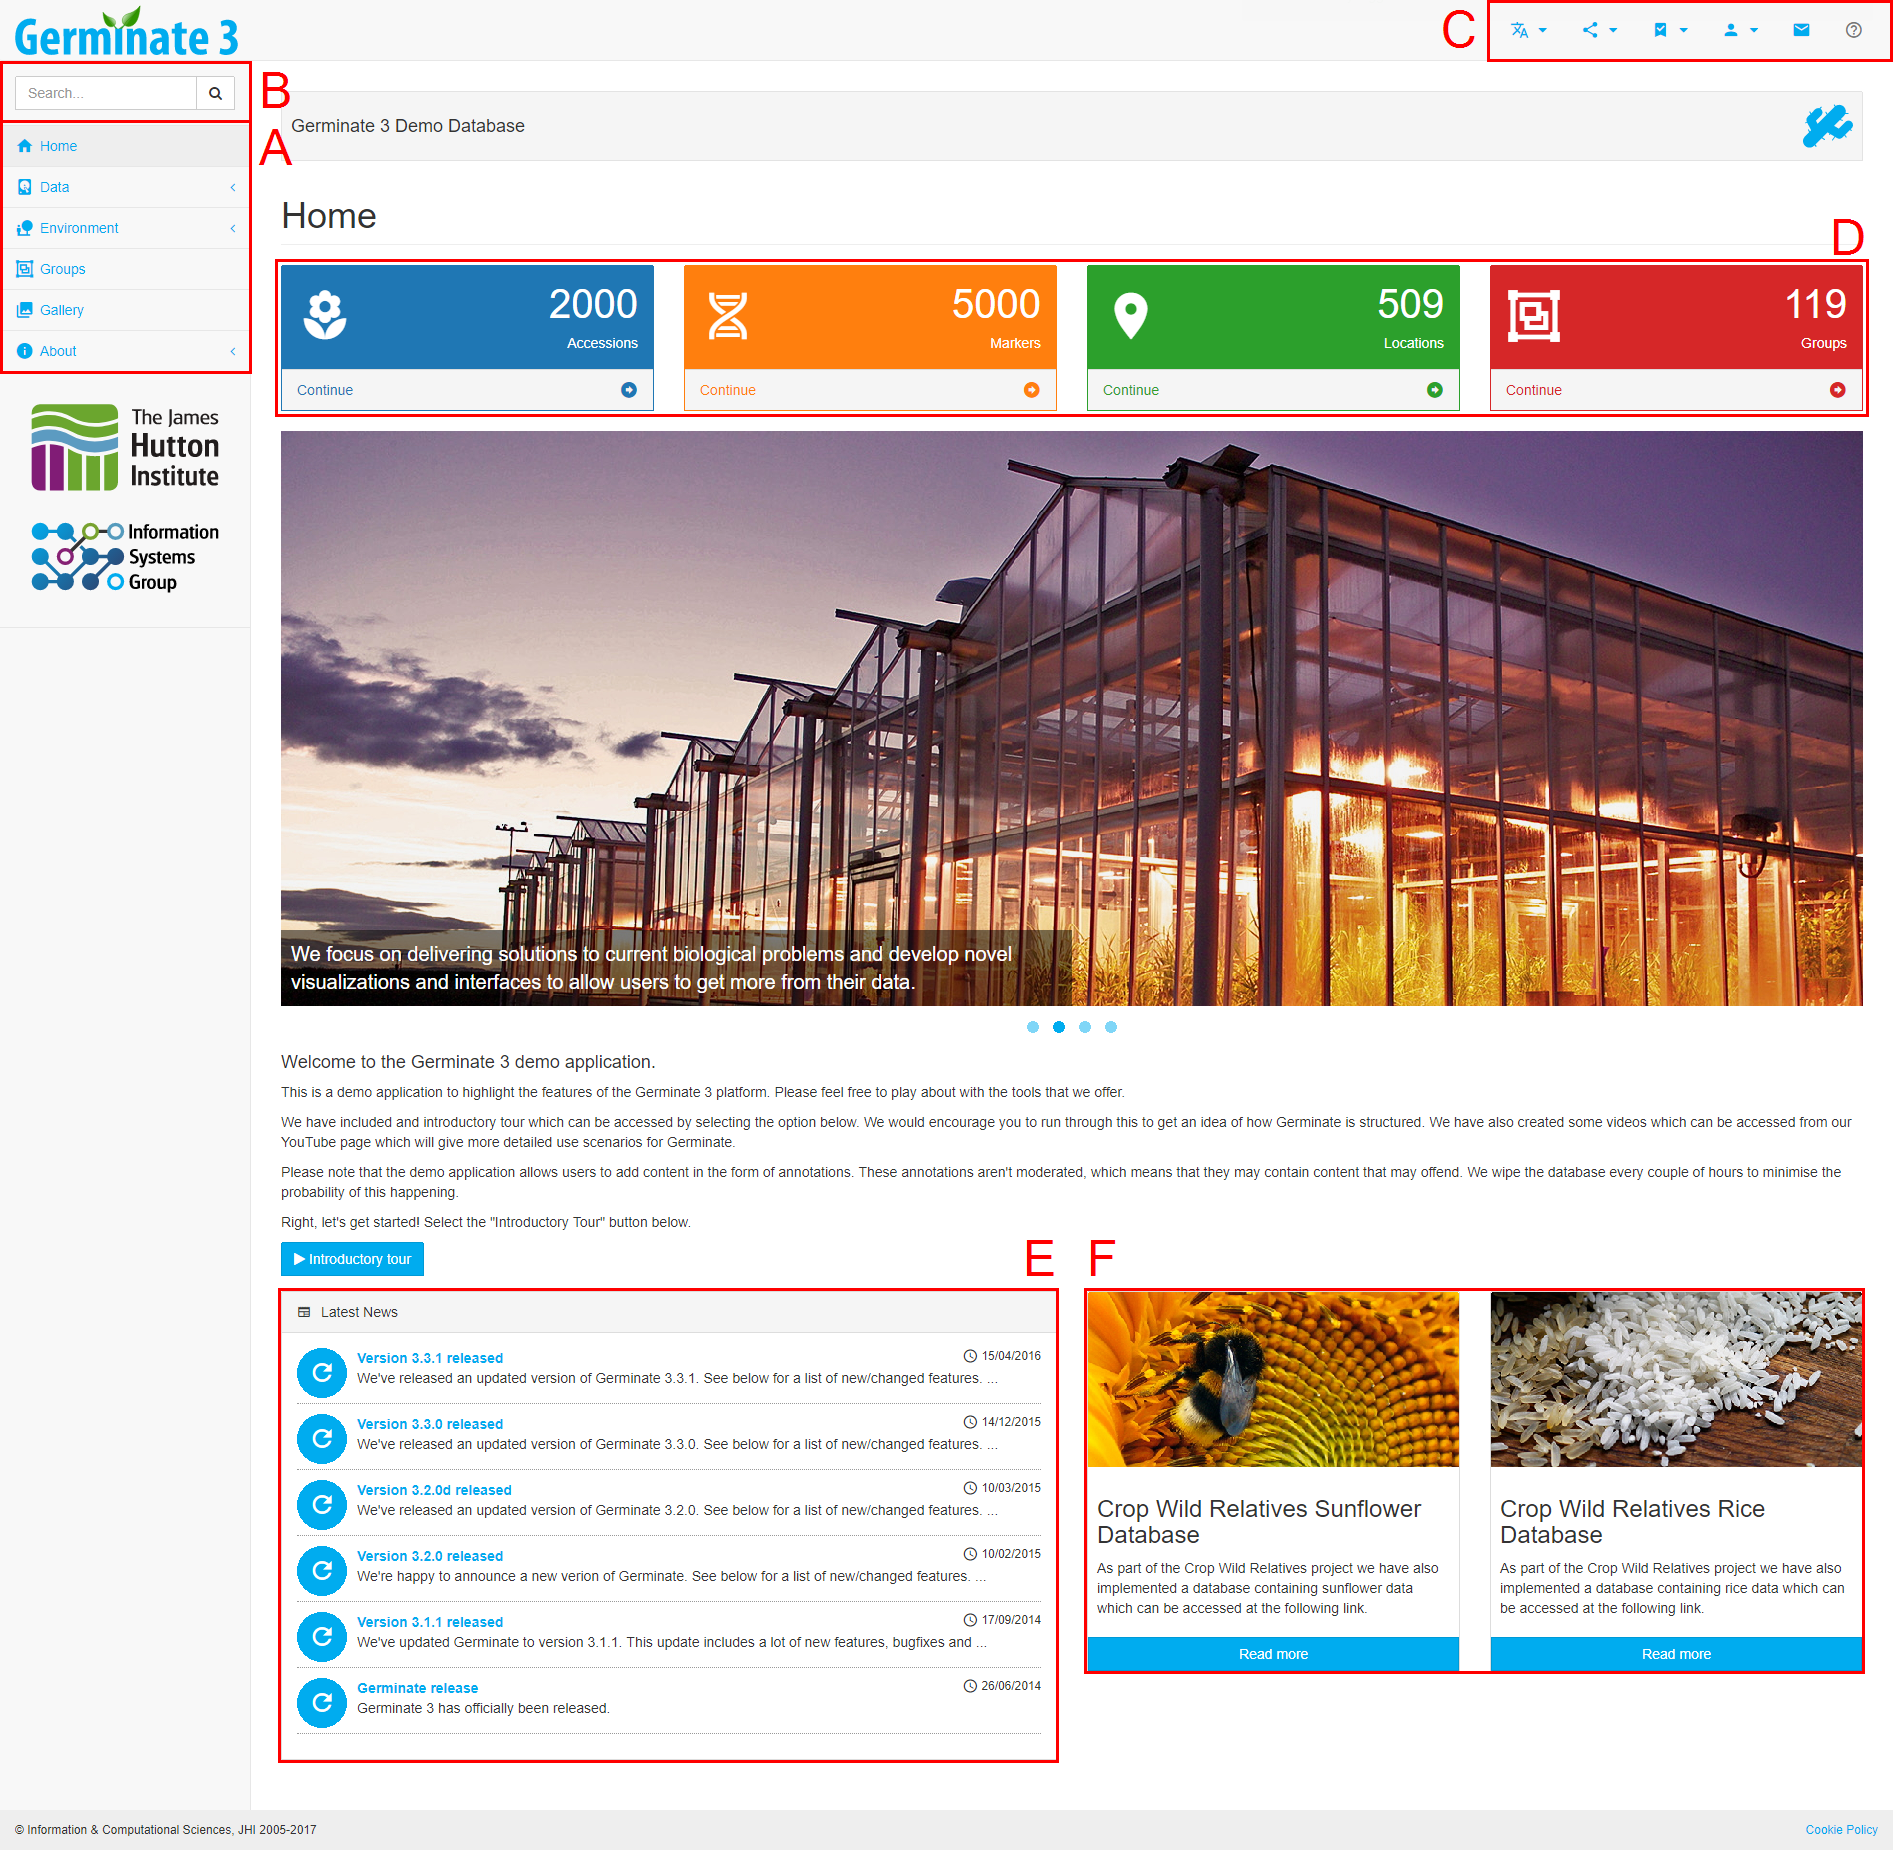
\includegraphics[width=0.85\linewidth]{img/overview/home.png}
	\caption{The home page of {\germinate} is the first page you will see. (A) The main menu of {\germinate} used to navigate the page. (B) The search box used for free-text searches of the database. (C) Language selector, social media buttons, marked item lists, user menu and the help button. (D) An overview of number of data objects that are stored in {\germinate}. (E) Latest news about this instance of {\germinate} and the contained data. (F) Other projects that have a relation to the current project.}
	\label{fig:overview:home}
\end{figure}